%! TEX root = 'main.tex'
\section{Experiment and Design}
\label{sec:implant-experiment}

\subsection{Reverse Engineering}
The PLC we use in this paper is Allen-Bradley 1769-L18ER-BB1B/B CompactLogix 5370. The reverse engineering process consists of two parts. The hardware part is primarily wire tracing, and the software part is to analyze the disassembly of the dumped firmware.

First, we need to determine each module in the PLC and check the microcontroller model and other essential IC chips. Next, we need to dump the firmware from the microcontroller and other chips.

\textbf{\textit{Backplanes.}} The Allen-Bradley CompactLogix 5370 contains several PCB module boards, known as backplanes. ~\autoref{fig:modules} shows that it contains one communication module, one real-time controller module, DC digital input/output module, and the power supply module. They are interconnected through proPrutoref{tab:memorymap} shows the memory map.ietary sockets.

The communication module \textbf{B} itself is a complete embedded system, including a CPU, DRAM, and other peripherals such as ethernet, SD card socket, and USB port. Its function is to communicate with the host to update firmware and ladder logic, and it also contains a web server. On the one hand, this module is not the one that controls IO, not our target. On the other hand, two FPGA chips are used to implement the processor and other peripheral devices such as the ethernet controller, making it very difficult to find the JTAG interface.

We focus on the real-time controller, which mainly executes the compiled ladder logic and controls the IO accordingly. Fortunately, the module uses a commercial microcontroller, Stellaris LM3S2793 SoC from Texas Instruments.

The IO module \textbf{D} has 16 inputs and 16 outputs socket, connecting to the real-time module \textbf{B}, through power switch and optically coupled isolator chips, eventually connected to the pins of the microcontroller. The LED module \textbf{E} contains LED lights for each IO socket and the status indicator of the PLC. Its wire goes through the communication module's PCB board and connects to the real-time module. Instead of directly connects each LED light, the microcontroller controls the LED module through the I2C protocol. The power module \textbf{A} provides stable 3 volts for other boards. The backdoor implant can either get power directly from it or the JTAG pad on the real-time module.

\begin{figure}[th]
	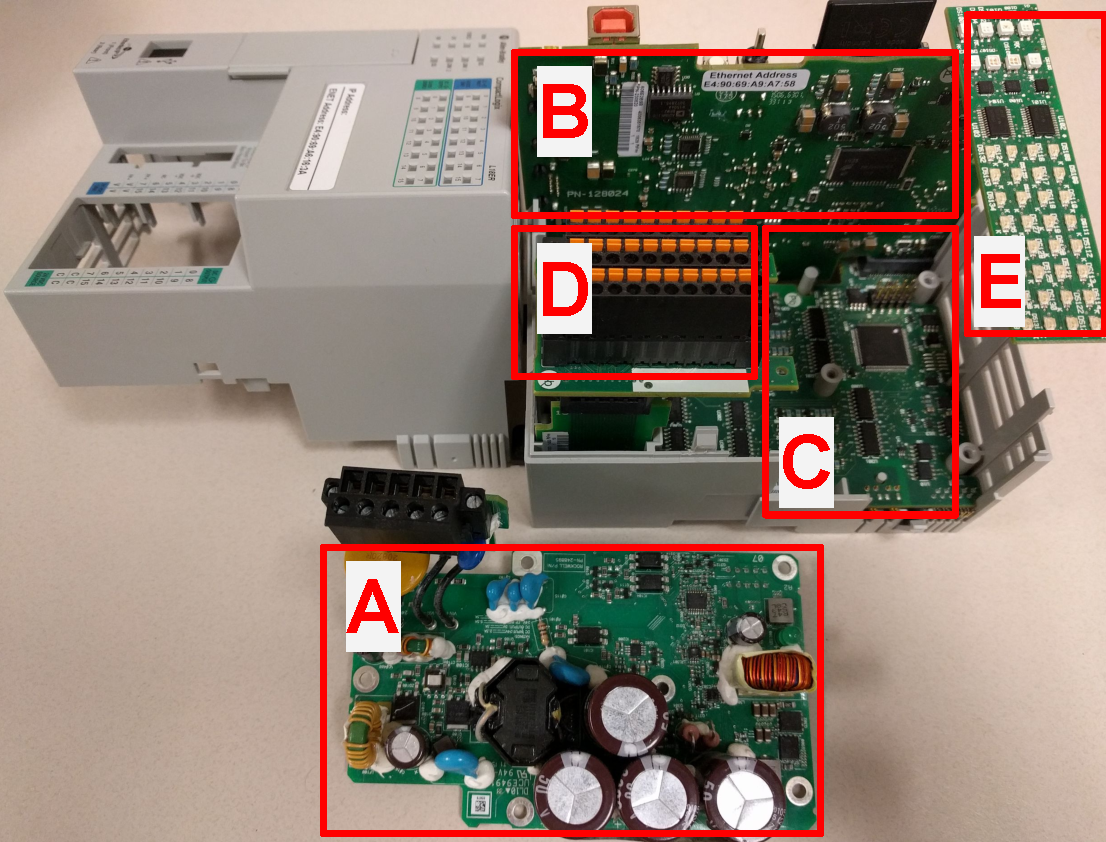
\includegraphics[width=0.47\textwidth]{figures/modules}
	\centering
	\caption{Allen-Bradley 1769-L18ER-BB1B/B CompactLogix 5370 PLC. A: Power supply module  B: Communication module  C: Real-time module  D: (16) DC Digital Outputs \& (16) DC Digital Inputs  E: LED indicator module}
	\label{fig:modules}
\end{figure}




\textbf{\textit{Microcontroller.}} The TI Stellaris LM3S2793 SoC has an ARM Cortex-M3 processor core that operates at 80 MHz. It contains 64 KB SRAM and 128 KB flash. The internal ROM is preprogrammed with Stellaris Peripheral Driver Library (DriverLib) to drive the on-chip peripheral devices. ~\autoref{tab:memorymap} shows the memory map. 


\begin{center}
	\begin{table}
		\begin{tabular}{|p{1.6cm} p{1.6cm} p{4cm}|} 
			\hline
			Start & End & Description \\ [0.5ex] 
			\hline
			0x00000000 & 0x0001FFFF & On-chip Flash \\ 
			\hline
			0x00020000 & 0x00FFFFFF & Reserved \\
			\hline
			0x01000000 & 0x1FFFFFFF & Reserved for ROM \\
			\hline
			0x20000000 & 0x2000FFFF & Bit-banded on-chip SRAM \\
			\hline
			0x20010000 & 0x21FFFFFF & Reserved \\
			\hline
			0x22000000 & 0x221FFFFF & Bit-band alias of bit-banded on-chip SRAM starting at 0x20000000 \\
			\hline
			0x22200000 & 0x3FFFFFFF & Reserved \\
			\hline
		\end{tabular}
		\caption{LM3S2793 Memory Map}
		\label{tab:memorymap}
	\end{table}
\end{center}



\textbf{\textit{Reset Vector.}} The vector table is fixed at address 0x00000000 on system reset. Once a core is out of reset sequence, it starts executing from memory address 0x00000004, the reset vector.  From the memory map, the reset vector resides in the flash memory instead of the ROM. The reason is that the ROM boot loader is only used as an initial program loader when the flash memory is empty and as an application-initiated firmware upgrade mechanism. For instance, if the data at address 0x00000004 is 0xFFFFFFFF, the ROM is mapped to address 0x00000000, and execution continues out of the ROM boot loader. If there is data at address 0x00000004 that is not 0xFFFFFFFF, the stack pointer (SP) is loaded from Flash memory at address 0x00000000 and the program counter (PC) is loaded from address 0x00000004. The firmware then begins executing from the flash memory.


In our case, the SP value is 0x20000B48, and the PC is 0x000000E3. Notice that 0xE3 is an odd number, ARM is a RISC architecture that uses a fixed-length instruction encoding format which uses four bytes instruction for the 32-bit processor. Certainly, the least significant bit indicates that the next branch uses Thumb instructions. Therefore we dump the flash memory and start to disassemble at address 0x000000E2.

\textbf{\textit{Flash boot loader.}} The SRAM is at 0x20000000. The flash boot loader copies itself to SRAM memory right after it starts, in consideration of performance. Even though the SRAM and flash memory can both be accessed in a single cycle, the manual says that the flash memory only can do that as long as the code is linear and branches incur a one-cycle stall. 

The code copies memory range 0x0 - 0xA88 to 0x20000000 - 0x20000A88 and initialize the data section 0x20000A88 - 0x20000F54 to 0.  Next, it uses the vector table that resides in SRAM. As mentioned above, on system reset, the vector table is fixed at address 0x00000000. The privileged code can write to the Vector Table Offset (VTABLE) register to relocate the vector table start address to a different memory location aligned on a 512-byte boundary. Replacing the vector table could mean completely changing the system's behavior because the corresponding interrupt vectors will point to different interrupt handlers to process peripheral devices' requests.


Finally, it sets the vector table to 0x20000000 and jumps to SRAM to continue.



\textbf{\textit{Stellaris Peripheral Driver Library.}} The Drivelib~\cite{lm3s2793rom} uses tables to provide library API entries. The tables have two levels. The main table contains one pointer per peripheral, which points to a secondary table containing one pointer per API associated with that peripheral. The main table is located at 0x01000010, right after the Cortex-M3 vector table in the ROM. \autoref{tab:romtable} shows a portion of the API table, and ~\autoref{tab:gpiotable} shows part of the ROM\_GPIOTABLE, which contains the entry points of all the GPIO related APIs.

\begin{center}
	\begin{table}
		\small
		\begin{tabular}{|p{7.2cm}|} 
			\hline
			ROM\_APITABLE (0x1000010) \\ [0.5ex] 
			\hline
			[0] = ROM\_VERSION \\
			\hline
			[1] = pointer to ROM\_UARTTABLE \\
			\hline
			[2] = pointer to ROM\_SSITABLE \\
			\hline
			[3] = pointer to ROM\_I2CTABLE \\
			\hline
			[4] = pointer to ROM\_GPIOTABLE \\
			\hline
			[5] = pointer to ROM\_ADCTABLE \\
			\hline
			... \\ 
			\hline
		\end{tabular}
		\caption{LM3S2793 ROM API Table}
		\label{tab:romtable}
	\end{table}
\end{center}

\begin{center}
	\begin{table}
		\small
		\begin{tabular}{|p{7.2cm}|} 
			\hline
			ROM\_GPIOTABLE \\ [0.5ex] 
			\hline
			[0] = function ROM\_GPIOPinWrite \\
			\hline
			[1] = function ROM\_GPIODirModeSet \\
			\hline
			[2] = function ROM\_GPIODirModeGet \\
			\hline
			[3] = function ROM\_GPIOIntTypeSet \\
			\hline
			[4] = function ROM\_GPIOIntTypeGet \\
			\hline
%			[5] = function ROM\_GPIOPadConfigSet \\
%			\hline
			... \\ 
			\hline
		\end{tabular}
		\caption{GPIO API Table}
		\label{tab:gpiotable}
	\end{table}
\end{center}


%The following is an example of calling function ROM\_GPIOPinRead() from the flash memory disassembly. API table indexing 0x1000010 + 0x10 (ROM\_APITABLE[4]) is optimized to 0x1000020 which points to the GPIO API table. [R2,\#0x2C] represents ROM\_GPIOTABLE[11] which is ROM\_GPIOPinRead(). So the code that calling the ROM library is very helpful to reveal the intent of the program.


\autoref{fig:romapiexample} shows a typical code snippet calling a ROM API. The table is at 0x1000010 + 0x10 (ROM\_APITABLE[4]), the GPIO table and the API is ROM\_GPIOPinRead() (ROM\_GPIOTABLE[11]). All the ROM API call sites have the same pattern, which makes reverse engineering the firmware much easier.  Calling the ROM API is merely to find the function address from the two-level tables and then jump to it. There is no privilege change; all the code runs in the system mode.


\begin{figure}[th]
	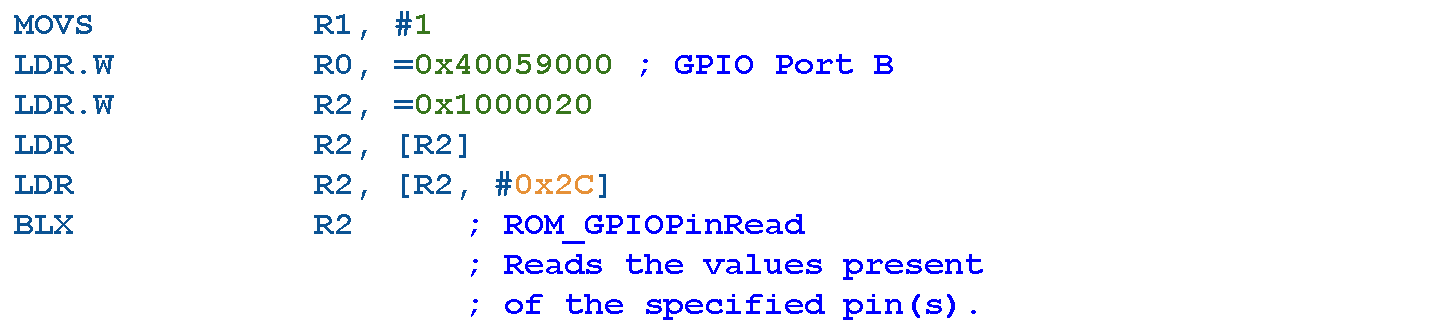
\includegraphics[width=0.47\textwidth]{figures/romapiexample2}
	\centering
	\caption{A code snippet calling ROM\_GPIOPinRead(). The parameters are passed in through the general registers where, in this case, the function has two parameters: R0 contains the GPIO port address to operate, and R1 is the bit-packed representation of the pins.  R2 stores the GPIO API table's address and eventually loads the API entry point and then jump to it.}
	\label{fig:romapiexample}
\end{figure}




\textbf{\textit{Debug.}} In addition to reverse-engineering,  we also need to debug the firmware. We use the SEGGER J-Link debugger. Since the target is ARM and the debugger sets up a GDB server, we also need GNU Embedded Toolchain for ARM~\cite{gnutoolchainarm}, an ARM version of the gdb client.


As mentioned earlier, the stack pointer and program counter are located at address 0x00000000 and 0x00000004. As shown in~\autoref{fig:gdbinit}, we use a GDB initialization script that contains GDB commands to set up the target. This script makes the PLC initialized and runs ladder logic, but the PLC cannot be interrupted during runtime with the debugger. If so, the indicator on the LED panel will prompt an IO error. The reason is still under investigation, and it could be that the watchdog timer is not handled well.

\begin{figure}[th]
	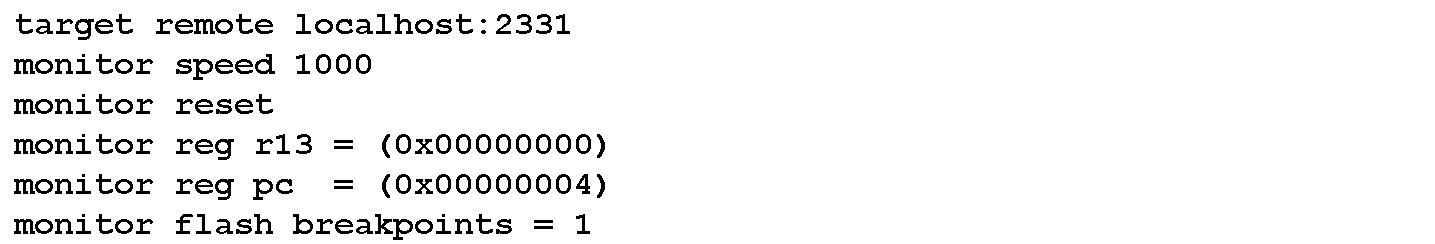
\includegraphics[width=0.47\textwidth]{figures/gdbinit}
	\centering
	\caption{The minimal gdbinit script that sets the SP and PC registers makes the PLC be up and running. Other on-chip peripheral controllers may not be correctly initialized.}
	\label{fig:gdbinit}
\end{figure}



%\subsubsection{more reverse engineering topics ....}

%Through reverse engineering, it shows that the Vector Table Offset Register is first at address 0x0, then switch to address 0x20000000, after receiving the ladder logic code, finally set to address 0x40000. 


\subsection{GPIO}

The hardware backdoor's essential function is to control the PLC's output to control the industrial physical system. The GPIO pins on the microcontroller either sensing the inputs or controls the outputs of the PLC.

For our target LM3S2793, the GPIO module comprises nine physical GPIO blocks, each corresponding to an individual GPIO port. Depending on the microcontroller's configuration, it supports up to 67 programmable input/output pins or several GPIOs grouped compose of a peripheral function such as I2C, and the GPIO ports can be accessed either through AHB or APB bus.  Each GPIO port has several associated control registers, such as GPIO Digital Enable (GPIODEN), GPIO Alternate Function Select (GPIOAFSEL), GPIO Port Control (GPIOPCTL), and GPIO Data Control registers. All GPIO pins are configured as GPIOs and tri-stated by default.

We primarily operate on the GPIO Data control registers. The GPIO Direction (GPIODIR) register configures each pin as an input or output, which should not be changed for the PLC's IO. The GPIO Data (GPIODATA) register modifies individual bits in GPIO ports. Different microcontrollers have their own operating methods on GPIOs, such as Output Data Register (ODR), Bit Reset Register (BRR), Bit Set/Reset Register (BSRR)~\cite{cottle2001programmable}. On LM3S2793, to modify individual GPIO pins in a single instruction without affecting the other pins' state, the operation on GPIODATA is not intuitive. Instead of each bit representing a GPIO pin,  it uses bits [9:2] of the address as a mask. Bits[1:0] are always zero because the memory access should be at 4-byte alignment on ARM.  For each GPIO port, it needs the memory range from GPIODATA to GPIODATA + 0x3FC to operate. If the address bit associated with that data bit is set during a write, the GPIODATA register's bit is altered. If the address bit is cleared, then the data bit is left unchanged.

For example, GPIO Port A (AHB) is at 0x40058000, and we want to set its bit-2 to 0 and bit-5 to 1. As shown in~\autoref{gpiowrite}, the address mask is 0x90, and the value we write is 0xF0.  Therefore, we need to write a value of 0xF0 to the address 0x40058090.

\begin{figure}[th]
	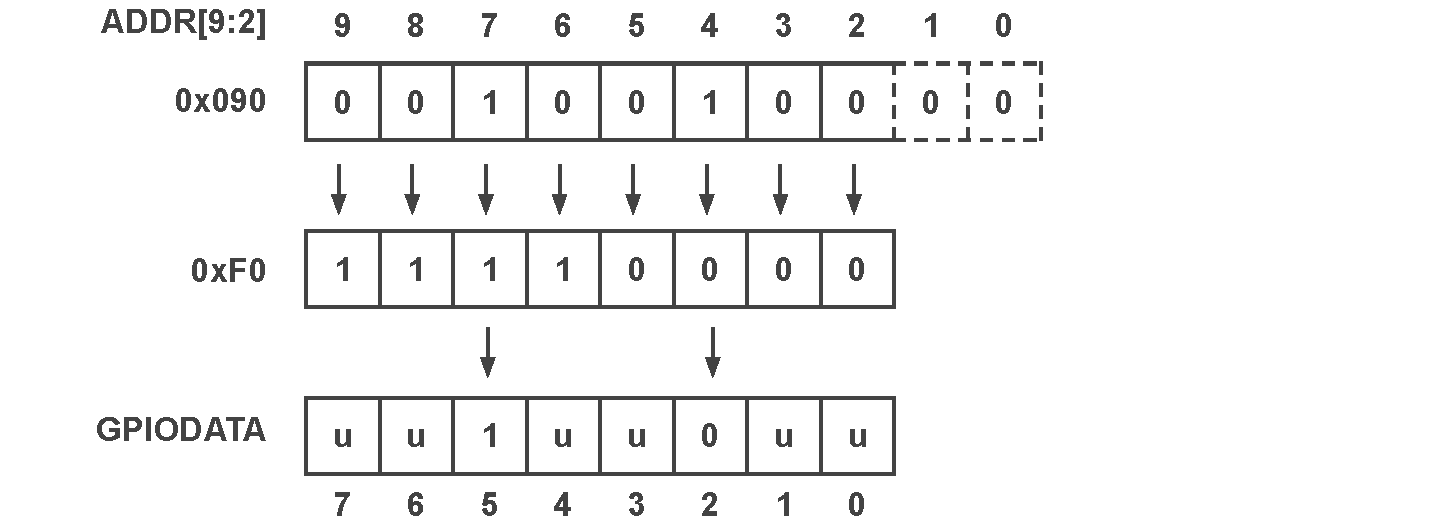
\includegraphics[width=0.47\textwidth]{figures/gpiowrite2}
	\centering
	\caption{GPIODATA Write Example. Writing a value of 0xF0 to the address GPIODATA + 0x090 has the bit-2 unset and bit-5 set in GPIODATA register where \textbf{u} indicates that data is unchanged by the write. Because of the mask, for example, writing 0xF0 or writing 0x2B has the same effect.}
	\label{fig:gpiowrite}
\end{figure}



To read a GPIO port, if the address bit associated with the data bit is set, the value is read. If the address bit associated with the data bit is cleared, the data bit is read as a zero, regardless of its actual value. For instance, we read GPIO Port A's high 4 bits. As shown in~\autoref{fig:gpioread}, the address mask is 0x3C0, and read address 0x400583C0 yields 0xA0.


\begin{figure}[th]
	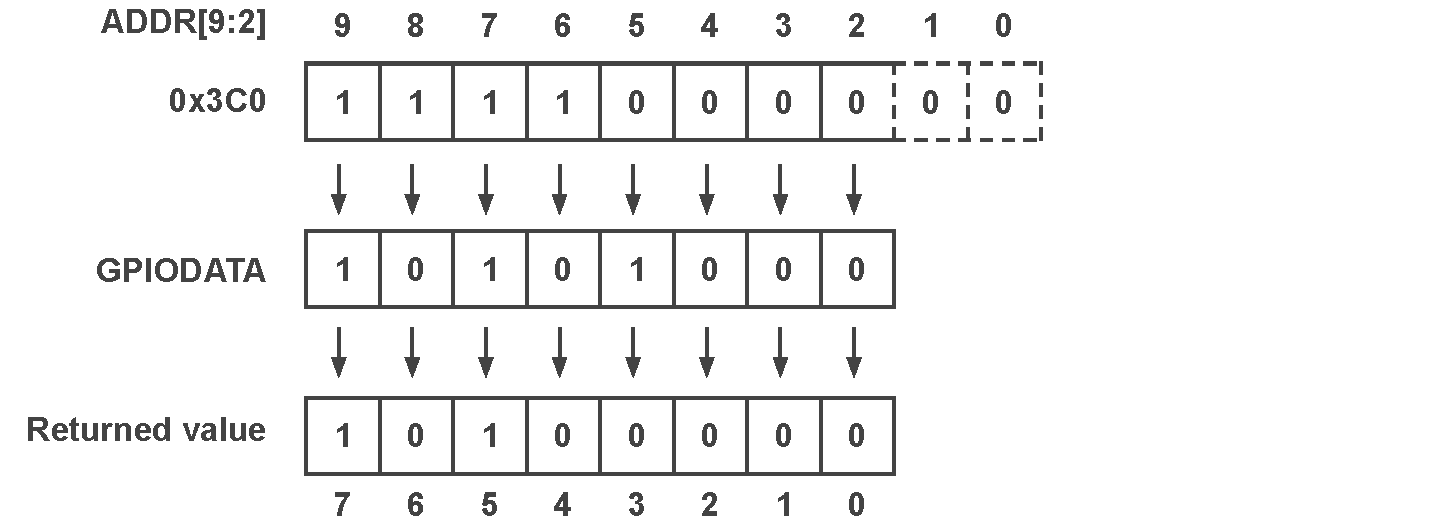
\includegraphics[width=0.47\textwidth]{figures/gpioread2}
	\centering
	\caption{GPIODATA Read Example. Reading address GPIODATA+0x3C0 returns the high 4 bits of the GPIO port because the address mask for the low 4 bits is all zeros.}
	\label{fig:gpioread}
\end{figure}



\subsection{Attacks}

To achieve a concealed attack on the PLC, we change its output without change the LED indicator on the front panel. More importantly, we have to ensure that the host side cannot detect any anomaly through the ladder logic.

There are 16 inputs and 16 outputs on the front panel. Through reverse engineering, we found the GPIO port corresponding to the input and output sockets. For example,  GPIO port E (0x4005C000), GPIO port F (0x4005D000) for inputs, and GPIO port G (0x4005E000), GPIO port H (0x4005F000) for outputs. Intuitively, each bit represents one pin, and 1 indicates the high voltage, which is the field power voltage that connects to the PLC; 0 dictates the low voltage (8 volts).

The PLC periodically scans the input, runs ladder logic, and updates output accordingly. It is called one scan cycle and implemented through a timer in the microcontroller. Following the timer handler routine, it is trivial to find the compiled ladder logic binary, and there are a few local variables that control its behavior. One local variable records if any logic state has changed. If so, the corresponding out GPIO port will be updated. We modify this local variable so that the output will not be updated from the ladder logic. Thus out attack can change the output arbitrarily without modifying the logic state. Doing so will not trigger any alarms.


\subsection{Other Onboard Components and Interconnections}

The methods mentioned above can satisfy a basic attack. To implement more complex attacks, we studied other components on the PLC boards.

\textbf{\textit{AT45DB021E SPI Flash Memory.}} There is an 8-pin chip
next to the LM3S2793 microcontroller. It is an Adesto 45DB021E 2-Mbit SPI flash memory chip and connected to the Synchronous Serial Interface (SSI0) of the microcontroller, as shown in ~\autoref{fig:ssi0}.


%Knowing how the real-time controller controls IO module, how to attack attack through the JTAG interface, we hope to learn more about the other chips on the board and how the different backplanes are related. We found that no other chips are daisy chained together with LM3S2793 via JTAG, so we need more reverse engineering work.

\begin{figure}[th]
	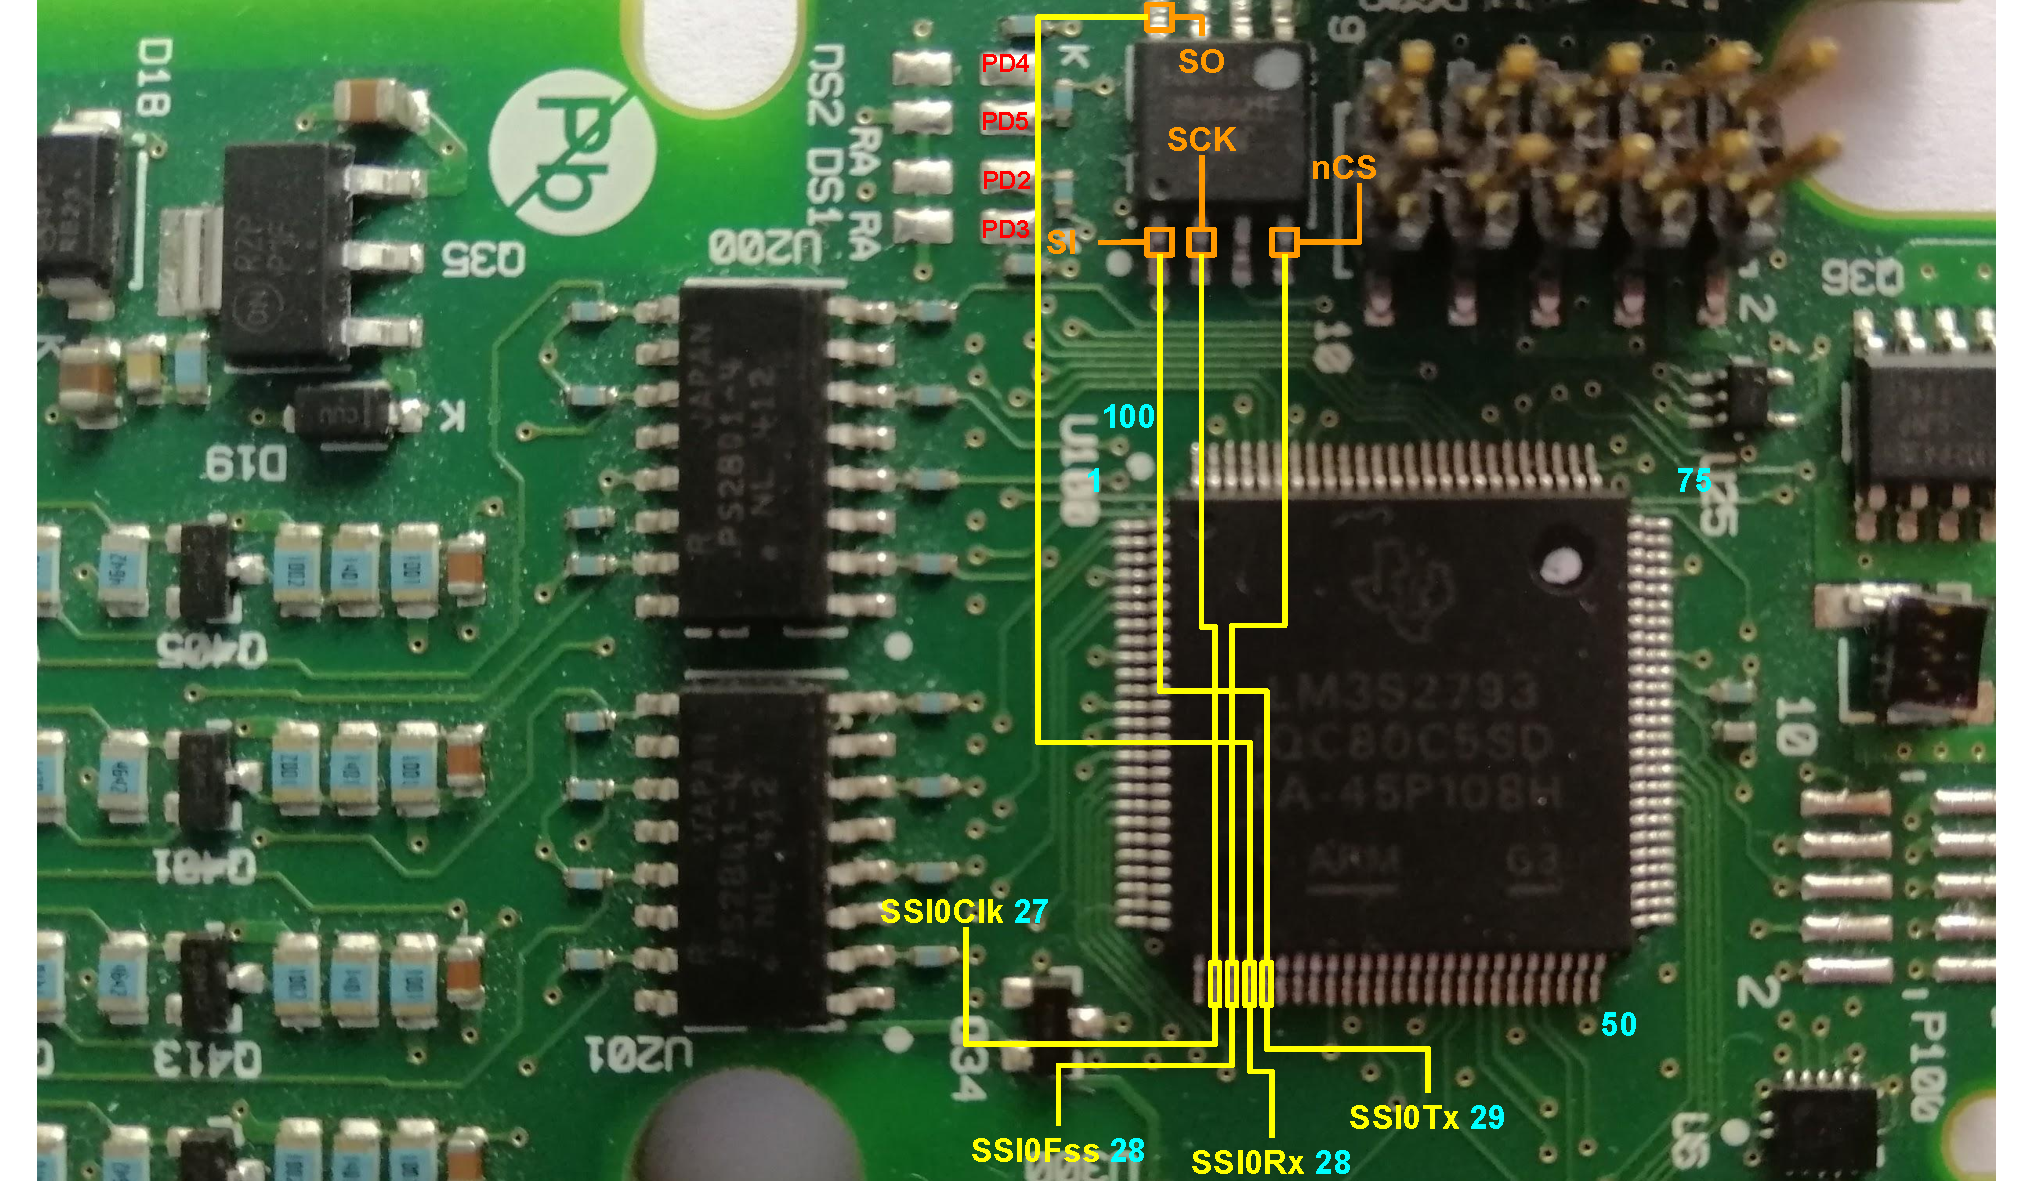
\includegraphics[width=0.47\textwidth]{figures/ssi0}
	\centering
	\caption{AT45DB21E SPI Flash Memory connects to LM3S2793's SSI0 interface. The pins on the 8-pin solder pad are also referenced in the firmware, but the device is not installed. It could be four LED indicators.}
	\label{fig:ssi0}
\end{figure}

%Also, at the beginning of the firmware initialization, right after copy part of the inner flash to RAM as we mentioned earlier, by associating GPIO port A and SSI0, the firmware first read a byte from the flash chip (at offset 0x2000). This byte is stored at address 0x20000F50. If the value of this byte is 0x55 or 0xAA, the firmware will reset the system, otherwise it will verify the firmware integrity from memory 0x4000 to 0x1FFFC. 

%The checksum is very simple. From 0x4000 to 0x1FFFC, accumulate each byte, and the final result is compared with the byte at 0x1FFFF. If they are equal, the check passes, otherwise, the firmware enters an infinite loop and keeps reset the watchdog.

%We can see that the variables saved in the external flash may indicate the state of the system's last run. Value 0x55 indicates something fatal happened. Right before it reset the system, the firmware setups 4 pins of GPIO port D as output and operates on it. We traced these 4 pins to a solder joint pad, as shown in~\autoref{fig:ssi0}, although this part is not installed.

%Value 0xAA indicates that the firmware from 0x4000 to 0x1FFFF is corrupted. The firmware reloads the partial image from external flash chip (from offset 0x6100) and sets variable 0x20000F50 to 0, then resets the PLC. But this image from AT45DB021E is a default backup.

In the boot loader, after jumping to SRAM, GPIO port A is assigned to the device SSI0. Then the firmware reads one byte from the flash chip (at offset 0x2000). If it equals either 0x55 or 0xAA, the firmware resets the PLC. Otherwise, the firmware starts to verify the integrity of the memory range 0x4000 to 0x1FFFC, which is the compiled ladder logic. The verification algorithm is a simple checksum. Each byte in this range is accumulated, and the final result should be equal to the byte of 0x1FFFF.

We think this byte in the flash memory represents the state of the last run.  A value of 0x55 indicates the system has encountered a severe error. The firmware then operates four pins from the GPIO port D, which leads to an empty 8-pin solder pad right next to the flash chip.  A value of 0xAA means that the ladder logic is corrupted, and data will be copied from the flash chip at offset 0x6100, which we believe is a backup.

To read the AT45DB21E flash chip's content, we port its driver to the Teensy 3.2 board. The source code is available at the github~\footnote{https://github.com/whensungoesdown/at45db021\_teensy32}. 




\textbf{\textit{Front Panel LED.}} There are four rows of LED lights on the PLC's front panel. Each LED shows individual input and output pins' status, which is an intuitive way for the administrator to check whether the device works properly. Underneath, the LED module \textbf{E} is controlled by the microcontroller through the I2C protocol~\cite{semiconductors2000i2c}. 

There are two 24-pin PD9535 mounted on module \textbf{E}. They are Remote 16-bit I2C and SMBus, Low-Power I/O Expander~\cite{pd9535}, which provides general-purpose I/O expansion for microcontrollers via the I2C bus. 

Two pins of GPIO port B (PB2 and PB3) are used as SCL and SDA by the I2C0 device on the microcontroller. Because module \textbf{E} connects both module \textbf{C} and module \textbf{E}, the SCL and SDA are found from the connector, as shown in~\autoref{fig:p607}


I2C slave device on the bus has a 7-bit unique address.  In this case, the two PD9535 chips for controlling input and output LED lights are assigned address 0x20 and 0x21, respectively.  Each of them has eight internal registers, as shown in~\autoref{tab:i2ccommand}. As mentioned in~\autoref{sec:background}, following the successful acknowledgment of the address byte, the microcontroller sends the command byte to select an internal register. 

Among the internal registers of PD9593, the configuration port registers configure the directions of the I/O pins. If a bit in this register is cleared to 0, the corresponding port pin is set as an output. The input port registers reflect the pins' incoming logic levels, regardless of whether the pin is defined as an input or an output by the configuration register. The output port registers set the outgoing logic levels of the pins. Since we use PD9593 to control LEDs, the pins are configured as outputs, and we do not need to read the input port registers. 

\begin{center}
	\begin{table}
		%\begin{tabular}{|c|@{}c@{}|c|c|} 
		\begin{tabular}{|@{}>{\centering\arraybackslash}m{0.8cm}@{}|
				@{}>{\centering\arraybackslash}m{3.25cm}@{}|
				@{}>{\centering\arraybackslash}m{2.30cm}@{}|
				@{}>{\centering\arraybackslash}m{1.5cm}@{}| }
			\hline
			\makecell{CMD \\Byte} & Register & Protocol & \makecell{Power-up \\Default}\\
			\hline
			0x00 & Input Port 0 & Read byte & xxxx xxxx\\ 
			\hline
			0x01 & Input Port 1 & Read byte & xxxx xxxx\\
			\hline
			0x02 & Output Port 0 & Read/Write byte & 1111 1111\\
			\hline
			0x03 & Output Port 1 & Read/Write byte & 1111 1111\\
			\hline
			0x04 & Polarity Inversion Port 0 & Read/Write byte & 0000 0000\\
			\hline
			0x05 & Polarity Inversion Port 1 & Read/Write byte & 0000 0000\\
			\hline
			0x06 & Configuration Port 0 & Read/Write byte & 1111 1111\\
			\hline
			0x07 & Configuration Port 1 & Read/Write byte & 1111 1111\\
			\hline
		\end{tabular}
		\caption{PD9535 internal registers can be selected by the command byte. To control LEDs, we only need to operate the control and output registers and keep the two polarity inversion registers' default values.}
		\label{tab:i2ccommand}
	\end{table}
\end{center}



\autoref{fig:ledi2cinit} shows the pseudo-code that uses ROM API to initialize one of the I2C IO expanders on the LED panel.  It first enables the I2C module and sets its clock, which should be the same as the microcontroller clock. After that, data is transferred by first setting the slave address using ROM\_I2CMasterSlaveAddrSet(). This function is also used to define whether the transfer is a read or a write. Then, the code calls the ROM\_I2CMasterDataPut() function with the data to send. The transaction starts when calling the ROMi\_I2CMasterControl(). In this case, 2 bytes of zero are sent to Configuration Port 0 and Port 1 sequentially, which sets the total 16 pins in output mode.


\begin{figure}[th]
	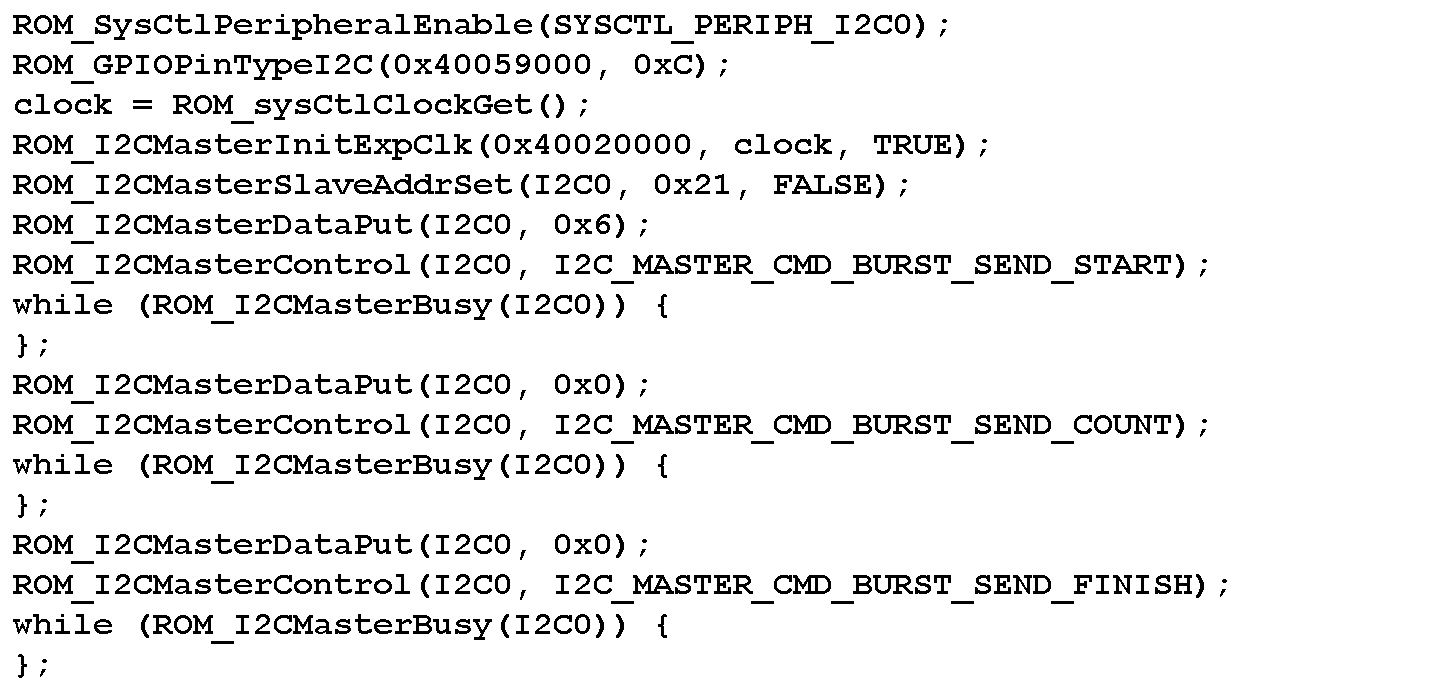
\includegraphics[width=0.47\textwidth]{figures/ledi2cinit}
	\centering
	\caption{The pseudo-code for initializing the I2C IO expander for LED lights is disassembled from the firmware. To make it easier to understand, we use the actual macros for some parameters, and their actual value is not difficult to find from the header files the vendor released.}
	\label{fig:ledi2cinit}
\end{figure}



After initialization, \autoref{fig:ledi2csend} shows how to control the LEDs. For instance, we send two bytes of 0xFF to the output port 0 and port 1, which lights up all 16 LEDs.


\begin{figure}[th]
	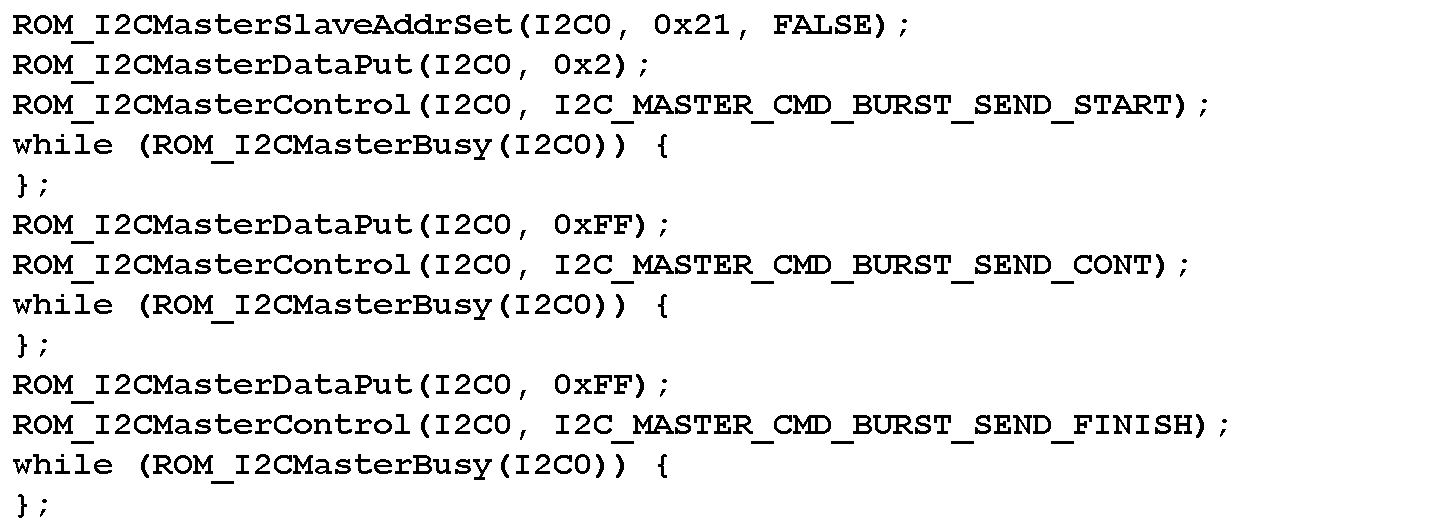
\includegraphics[width=0.47\textwidth]{figures/ledi2csend}
	\centering
	\caption{Each pin of the output port 0 and port 1 control one LED, respectively. Therefore two 0xFF will light all the 16 LEDs up. To only set one register, we also can call  ROM\_I2CMasterControl() with parameter I2C\_MASTER\_CMD\_SINGLE\_SEND.}
	\label{fig:ledi2csend}
\end{figure}





\textbf{\textit{Onboard Connectors.}}

There are several connectors on the module \textbf{B}, as shown in~\autoref{fig:board}. P607 is the one that connects to the communication board (module \textbf{B}), and p609 connects to the power board (module \textbf{A}). We comprehend some of these pins' functions through continuity tests with a multimeter, as shown in~\autoref{fig:p607}. In addition to the I2C bus, there is also a CAN bus passing through this connector. In this way, both module \textbf{B} and module \textbf{C} connect to the same CAN bus connector as shown at the bottom of~\autoref{fig:board}. On the microcontroller LM3S2793, the other end is the CAN0 device with pin PA6 and PA7. However, the communication board has higher authority; it can prohibit signal transmission on RxD (pin 21) by setting pin 29 to 1.

\begin{figure}[th]
	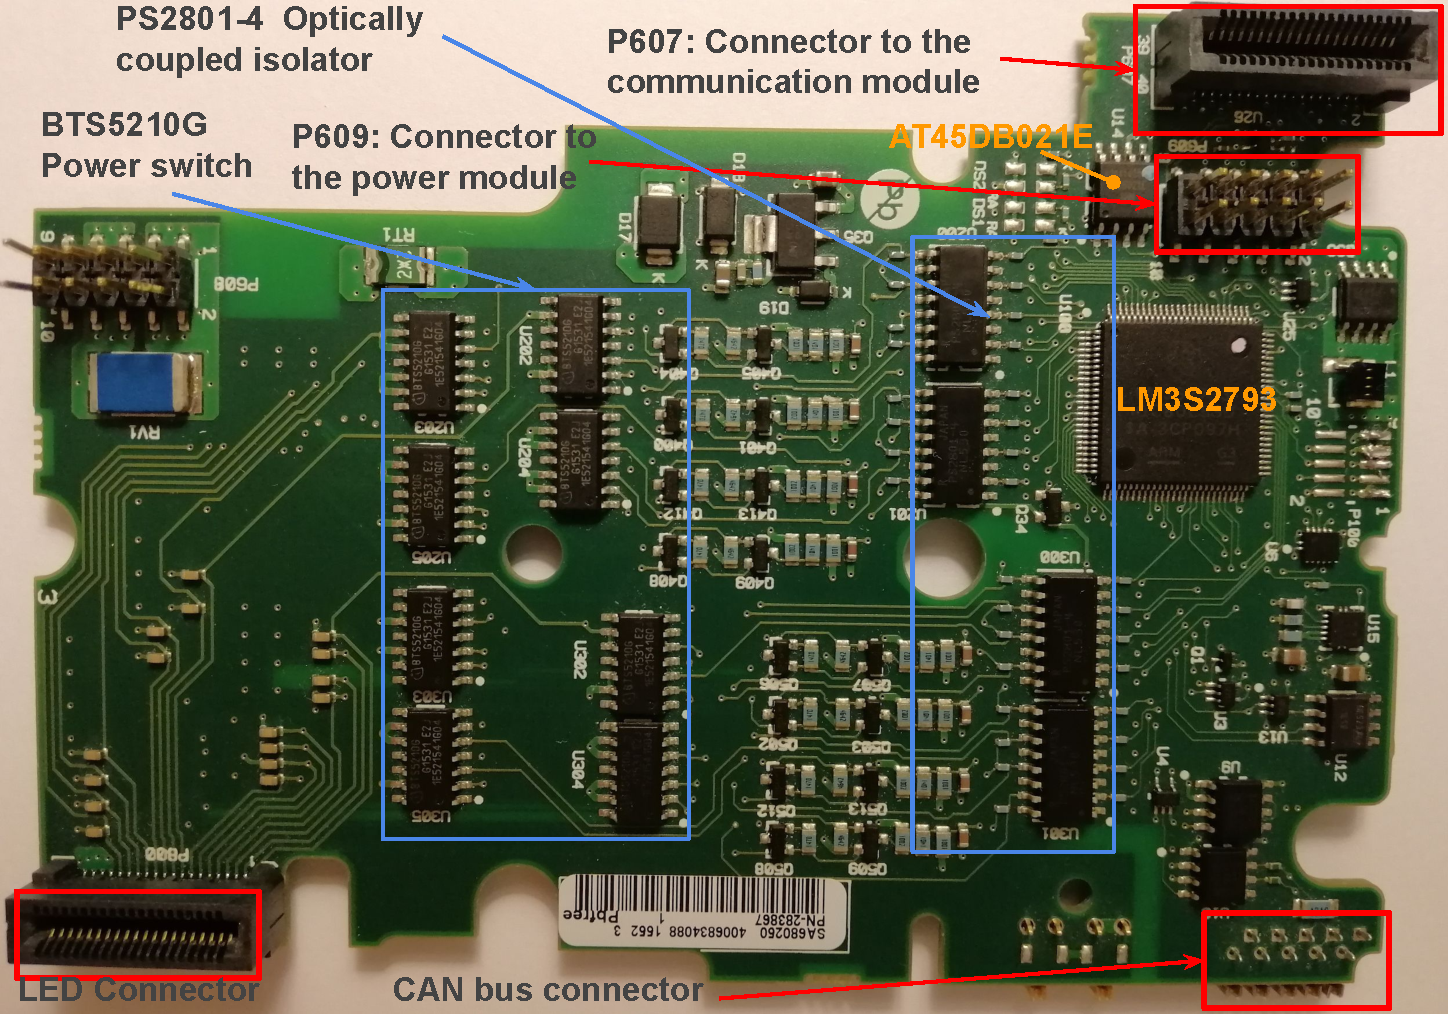
\includegraphics[width=0.47\textwidth]{figures/board2}
	\centering
	\caption{The real-time board reads the inputs, runs compiled ladder logic binary, and drives the outputs. It is the board that interconnects all other modules. Besides the microcontroller and the flash memory, there are power regulators and IO chips. The optically coupled isolators prevent high voltages from affecting the microcontroller receiving the signal, and the power switches provide the electrical connection between the output pin and the voltage source.}
	\label{fig:board}
\end{figure}


\begin{figure}[th]
	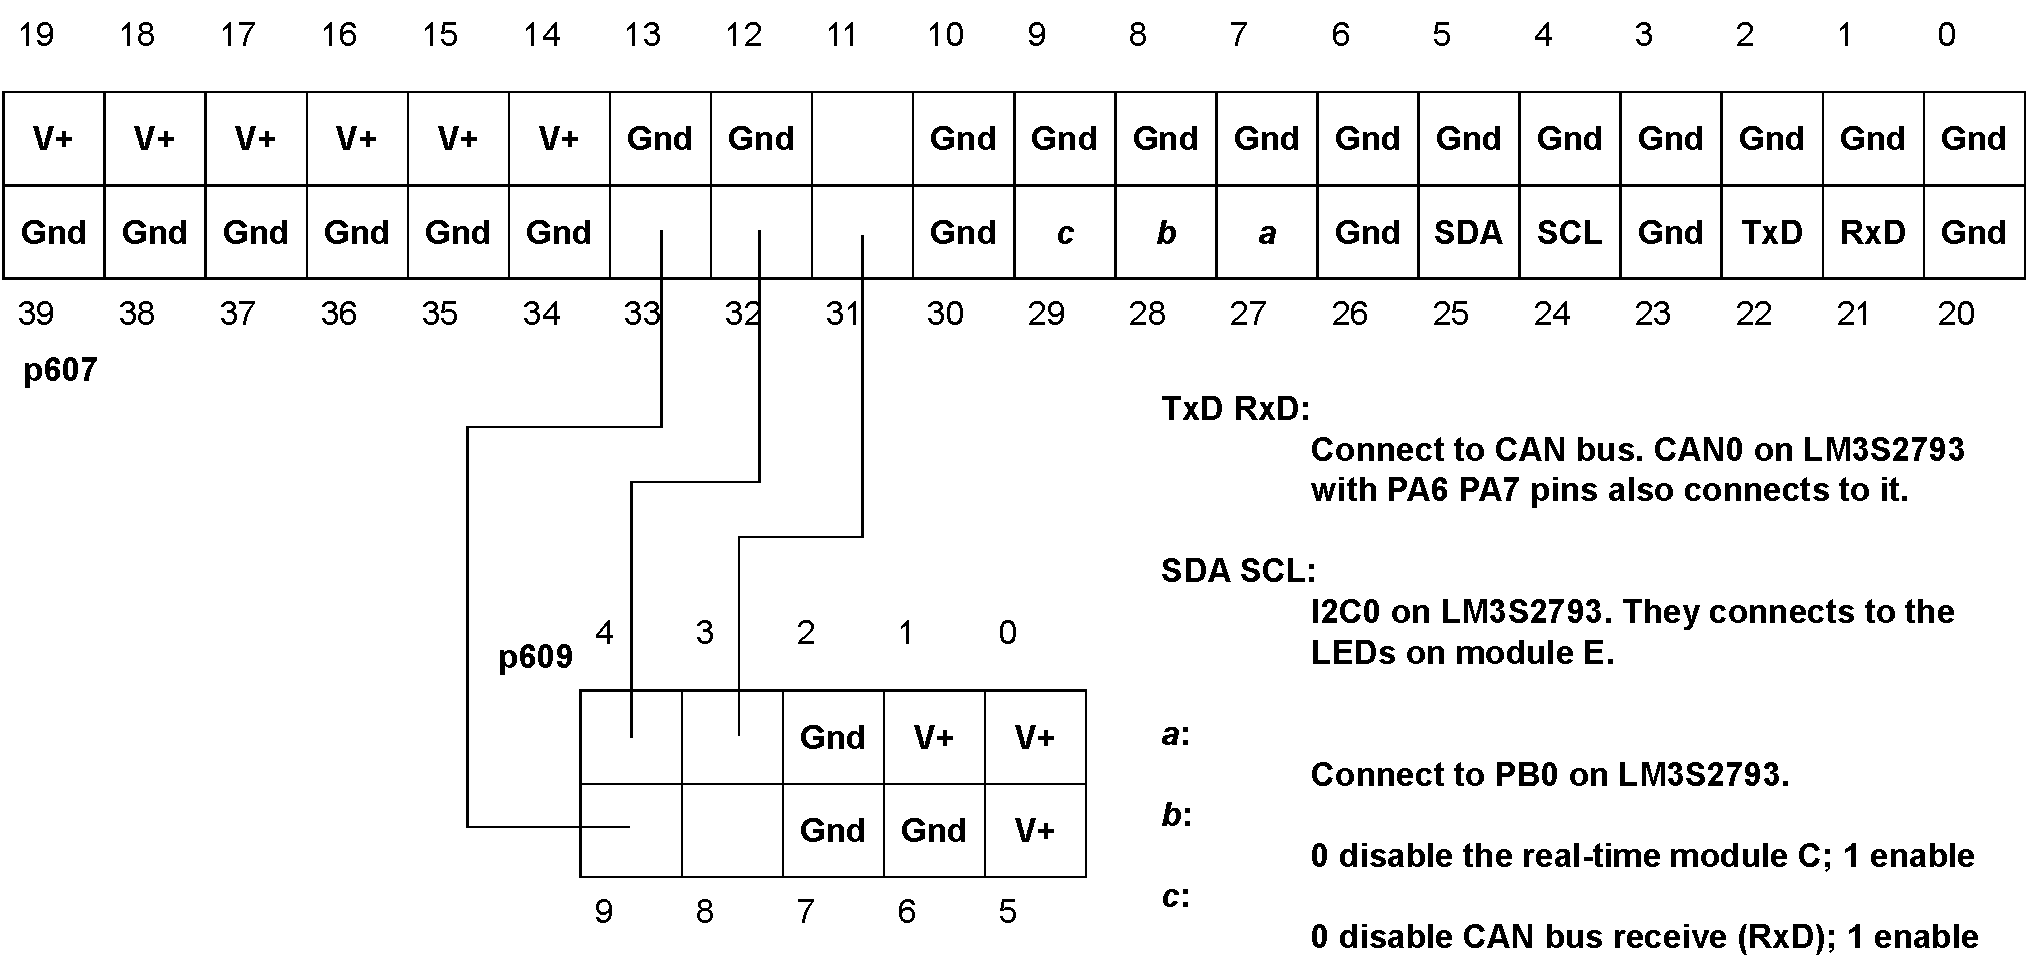
\includegraphics[width=0.47\textwidth]{figures/p607_2}
	\centering
	\caption{The connector between the communication board (module \textbf{B}) and real-time board (module \textbf{C}) comprises the I2C bus and CAN bus. }
	\label{fig:p607}
\end{figure}

%As mentioned earlier, on module C, there is a AT45DB21E flash chip. It connects to the microcontroller through SSI0. And it contains one copy of code that will be loaded in once the microcontroller is caught in an unrecoverable error. But by analyzing this interface, we found that the communication module B is not connected to this AT45DB21E flash chip. So we think the code in it is just the backup code used to recover from the fatal error state, and the updated compiled ladder logic is updated by other means.  
%
%By reverse engineering the circuit board and firmware, we identified pin 24 and pin 25 of the connector as the SCL and SDA pin of I2C bus, as shown in~\autoref{fig:p607}. The microcontroller LM3S2793's PAxx PAxx connects LED module E through the communication module B, as shown in~\autoref{fig:modules}.
%
%We also identified that pin 21 and pin 22 are used as CAN bus input and output that come from the communication module B. And pin 29 is used to disable the CAN bus receive signal (RxD). On the CompactLogix PLC 1766, there is only one set of CAN bus for connecting modules. It located on the side of the PLC, it's part of the real-time module, as shown in~\autoref{fig:board}.
%
%
%Both the communication module B and real-time module C are connected to this bus.


\subsection{Design}

Typically, the PLC has a dedicated real-time microcontroller
that handles IO, in this case, module \textbf{D}. It runs minimal code, mainly the compiled ladder logic.  To receive ladder logic update, the communication module \textbf{C} talks to the HMI and then update the real-time microcontroller through the CAN bus. Therefore, to remotely control the PLC's IO, the attacker needs to control further the communication module \textbf{C}, which itself is an independent system usually with a more powerful processor. Moreover, an abnormal traffic filtering mechanism~\cite{kim2016abnormal} also may be deployed to protect ICS networks. Even though we successfully controllers all the embedded system in the PLC and penetrates the network traffic monitors, we still have to face the challenge that a critical infrastructure may run on an isolated local network. Therefore, we choose to use a separate network using GSM.

\begin{figure}[th]
	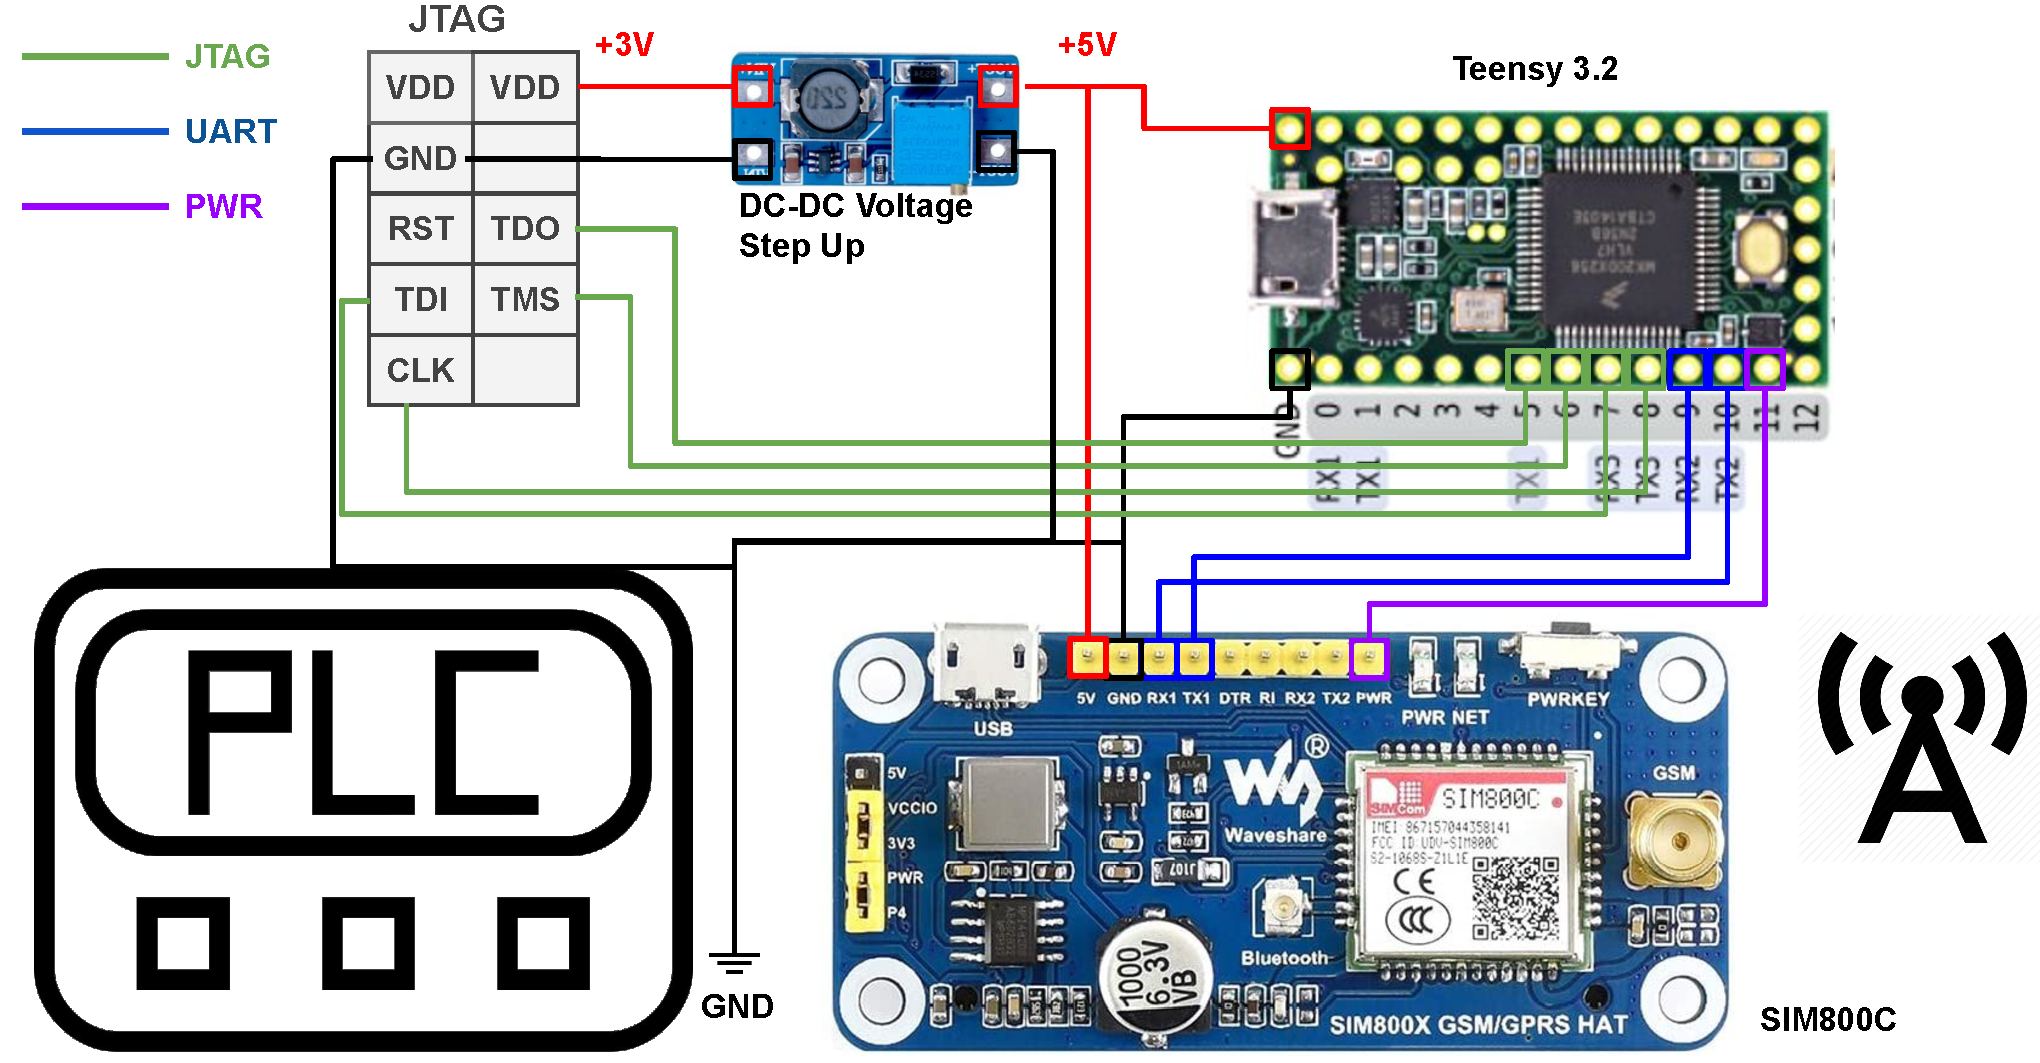
\includegraphics[width=0.47\textwidth]{figures/sim800teensy}
	\centering
	\caption{The power can be drawn from the JTAG pad or directly from the border connector p607. Since the JTAG pad provides the 3 volts source, we also need a DC-DC voltage step-up module that boosts from 3 volts to 5 volts. One GPIO pin from Teensy connects the PWR pin of the SIM800C board. It is used to deliver the power and reset sequence. After SIM800C initialized, the Teensy module sends AT commands through the serial port.}
	\label{fig:sim800teensy}
\end{figure}

The SIM800C is a Quad-Band GSM/GPRS module. It has strong extension capability with interfaces including UART, USB2.0, and GPIO. ~\autoref{fig:sim800teensy} shows that the SIM800C module connects with the Teensy board through a serial port. First, the Teensy boart initializes the cellular module using AT command, connecting to the network. Once a text message is received, the Teensy board reads it and looks for control commands. In such a case,  the command will be parsed as IO operations that eventually turn into particular memory read/write on PLC's GPIO port.
